\documentclass[12pt, a4paper]{article}

\usepackage[utf8]{inputenc}
%\usepackage[spanish]{babel}
\usepackage{amsmath}
\usepackage{amsfonts}
\usepackage{amssymb}
\usepackage{graphicx}
\usepackage{float}
\usepackage{listings}
\usepackage{multirow}

\usepackage[left=2cm,right=2cm,top=2cm,bottom=2cm]{geometry}

\author{5175: \'Angel Moreno \\ Tarea \# 4: Complejidad asintótica experimental}
\title{Optimizaci\'on flujo en redes}

\begin{document}
\maketitle

Se utiliza los siguients generados de grafo:
\begin{enumerate}
	\item complete\_graph
	\item circulant\_graph
	\item wheel\_graph
\end{enumerate}
para crear 10 grafos de dimensiones 32, 64, 128 y 256, ponderados con una distribuci\'on $\sim \mathcal{N}(10, 1)$. Para cada uno de los grafos generados se implementa los siguientes algoritmo de flujo m\'aximo:
\begin{enumerate}
	\item maximum\_flow
	\item preflow\_push
	\item shortest\_aumenting\_path
\end{enumerate}
se ejecutan con 5 diferentes fuentes y sumideros un total de 5 r\'eplicas. Se toma el tiempo de ejecuci\'on de la implementaci\'on y se hace un an\'alisis estad\'istico contra los diferentes factores cantidad de nodos, densidad del grafo, algoritmo de generaci\'on y algoritmo de flujo m\'aximo.

\section{Resultados}

La figura \ref{fig: generador} muestra la caja bigotes de generadores grafos contra tiempo de ejecuci\'on, se observa en el bloque del generador del grafo completos tiempo de ejecuci\'on son m\'as altos que los dem\'as algoritmo. La figura \ref{fig: algoritmo} muestra el gr\'afico de los algoritmos de flujo m\'aximo contra el tiempo de ejecuci\'on, se observa que el tiempo de ejecuci\'on del algoritmo depende del grafo. La figura \ref{fig: orden} muestra que el tiempo de ejecuci\'on aumenta seg\'un el orden del grafo y la figura \ref{fig: densidad} se observa que el entre mas densidad mas afecta ene le tiempo de ejecuci\'on.
\begin{figure} [H] \centering
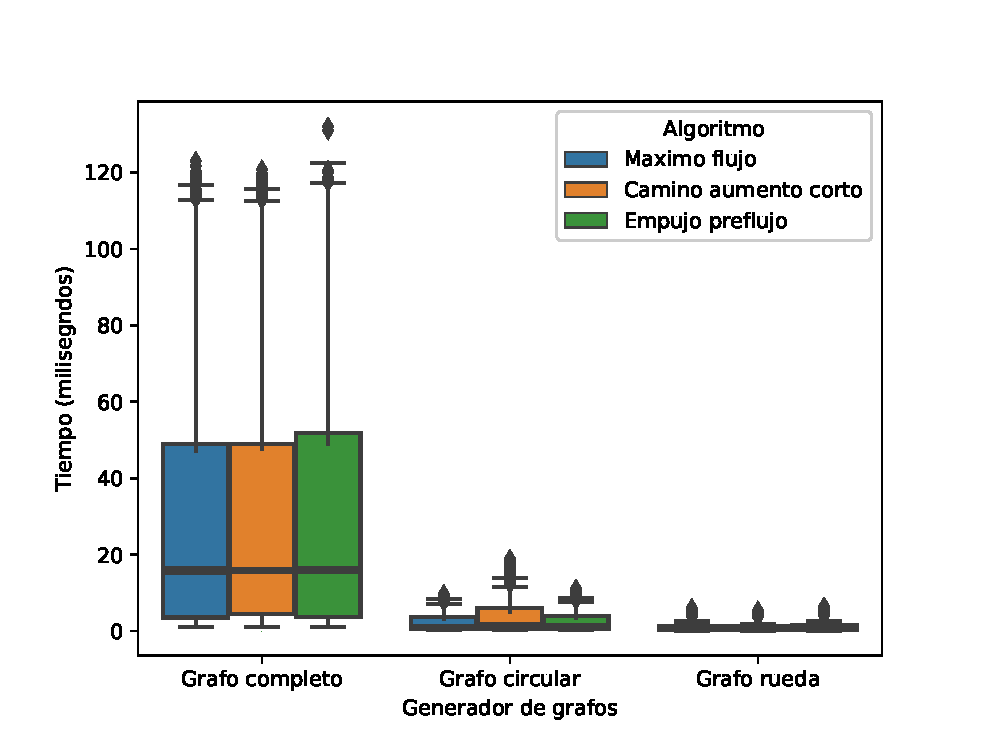
\includegraphics[scale=0.8]{figura1}
\caption{Efecto del geneador de grafos contra tiempo de ejecuci\'on.}
\label{fig: generador}
\end{figure}

\begin{figure} [H] \centering
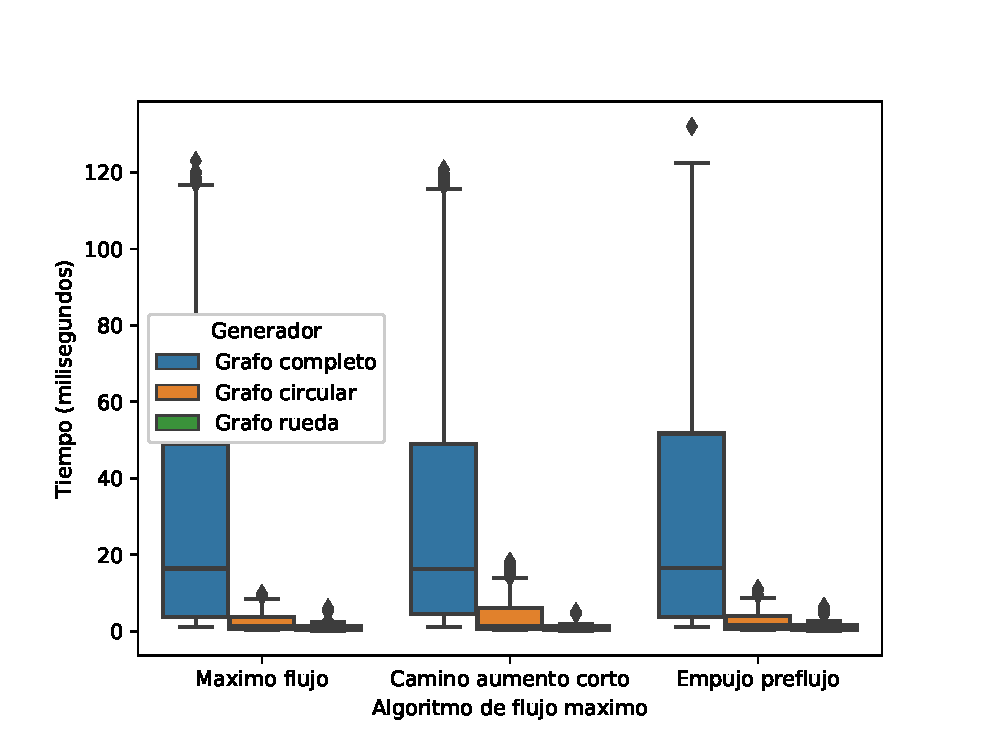
\includegraphics[scale=0.8]{figura2}
\caption{Efecto del algoritmo contra tiempo de ejecuci\'on.}
\label{fig: algoritmo}
\end{figure}

\begin{figure} [H] \centering
\includegraphics[scale=0.8]{figura3}
\caption{Efecto del orden del grafo contra el tiempo de ejecuci\'on.}
\label{fig: orden}
\end{figure}

\begin{figure} [H] \centering
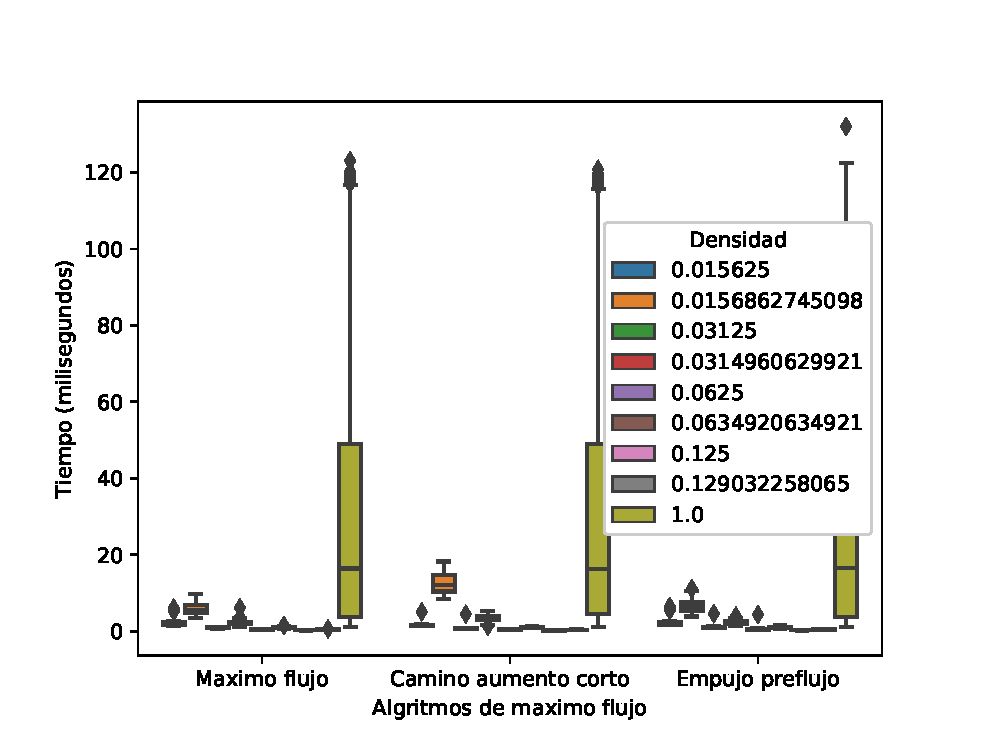
\includegraphics[scale=0.8]{figura4}
\caption{Efecto de la densidad del grafo contra tiempo de ejecuci\'on.}
\label{fig: densidad}
\end{figure}


\begin{table}[H]
\begin{center} \begin{tabular}{|lrrrr|}
\hline
Factor & Cuadrados medios & GL & $F$ & $F_{GL}$ \\ \hline \hline
Generador           &   4236.598736  &    2.0 &     56.139347 &   2.271267e-24 \\ \hline
Algoritmo           &    103.331225  &    2.0 &      1.369246 &   2.545659e-01 \\ \hline
Generador:Algoritmo &    368.019017  &    4.0 &      2.438318 &   4.518991e-02 \\
Orden               & 779151.982887  &    1.0 &  20649.150964 &   0.000000e+00 \\
Generador:Orden     &    844.240482  &    2.0 &     11.187066 &   1.485138e-05 \\ \hline
Orden:Algoritmo     &     49.606236  &    2.0 &      0.657334 &   5.183566e-01 \\ \hline
Densidad            &  69967.332330  &    1.0 &   1854.280089 &  2.725925e-278 \\
Generador:Densidad  &    399.506210  &    2.0 &      5.293873 &   5.101561e-03 \\ \hline
Algoritmo:Densidad  &     73.938648  &    2.0 &      0.979764 &   3.756018e-01 \\ \hline
Orden:Densidad      &    155.993981  &    1.0 &      4.134166 &   4.217371e-02 \\
Residual            &  67239.996255  & 1782.0 &           	  &            	  \\
\hline
\end{tabular} \end{center}
\caption{Analisis de varianza de los factores.}
\label{tab:resultados}
\end{table}

El cuadro \ref{tab:resultados} muestra el an\'alisis de varianza y se observa que el algoritmo, orden-algoritmo y densidad-algoritmo infuyen en el tiempo de ejecuci\'on, mientras que los dem\'as factores no afecta el tiempo de ejecuci\'on.

\begin{thebibliography}{X}
\bibitem{elisa} \textsc{Schaeffer E.} \textit{Optimización de flujo en redes, 2019.} \\
\texttt{https://elisa.dyndns-web.com/teaching/opt/flow/}
\bibitem{lalo} \textsc{Kamada T.} \textit{An Algorithm for Drawing General Undirected Graphs} \\
\texttt{Information Processing Letters, 1988.}
\bibitem{lili} \textsc{Saus L.} \textit{Repository of Github, 2019.} \\
\texttt{https://github.com/pejli}
\end{thebibliography}


\end{document}